\documentclass[12pt,a4paper,%
%draft%
]{scrreprt}
% prevent warning \float@addtolists detected
\usepackage{scrhack} 

% Textkodierung Deutsch
\usepackage[ngerman]{babel}
\usepackage[T1]{fontenc}
\usepackage[utf8]{inputenc}
\usepackage{lmodern}
\usepackage{xspace}
\usepackage{microtype}

% Basisinfos
\title{Modellbasierte Testautomatisierung eines verteilen, adaptiven Load-Balancing-Systems}
\author{Gerald Siegert}
\date{\today}
%Variablen welche innerhalb der gesamten Arbeit zur Verfügung stehen sollen
\newcommand{\titleDocument}{Masterarbeit}
\newcommand{\subjectDocument}{im Studiengang Informatik}
\newcommand{\zB}{z.\,B. }
\newcommand{\uA}{u.\,A. }
\newcommand{\sS}{S\# }
\newcommand{\cS}{C\# }
\newcommand{\uU}{unter Umständen}
%hier müssen alle Wörter rein, welche Latex von sich auch nicht korrekt trennt bzw. bei denen man die genaue Trennung vorgeben möchte
\hyphenation
{
    Film-pro-du-zen-ten
    Lux-em-burg
    Soft-ware-bau-steins
    zeit-in-ten-siv
}
\renewcommand{\texttt}[1]{%
    \begingroup
    \ttfamily
    \begingroup\lccode`~=`/\lowercase{\endgroup\def~}{/\discretionary{}{}{}}%
    \begingroup\lccode`~=`[\lowercase{\endgroup\def~}{[\discretionary{}{}{}}%
    \begingroup\lccode`~=`.\lowercase{\endgroup\def~}{.\discretionary{}{}{}}%
    \catcode`/=\active\catcode`[=\active\catcode`.=\active
    \scantokens{#1\noexpand}%
    \endgroup
}

% Seitenränder
\usepackage{geometry}
\geometry{left=35mm,right=20mm,top=25mm,bottom=20mm}

% Kopf/Fußzeilen
\usepackage[headsepline]{scrlayer-scrpage}
\clearscrheadfoot
\pagestyle{scrheadings}

\ihead{\headmark}
\automark{chapter}
\ohead{\pagemark}

\renewcommand*{\headfont}{\normalfont}
\setlength{\headheight}{1.5\baselineskip}
\renewcommand*{\chapterpagestyle}{scrheadings}

\newpairofpagestyles[scrheadings]{lists}{%
    \ihead{Verzeichnisse}%
    }

% Grafiken
\usepackage{graphicx}
\usepackage{wrapfig}
\usepackage[format=plain]{caption}
\setkeys{Gin}{width=0.8\columnwidth} % default width
% Markow-Ketten
\usepackage{tikz}
\usetikzlibrary{automata,positioning,arrows}
 
% Tabellen
\usepackage{multirow}

% Textfarben
\usepackage{xcolor}

% Abkürzungen
\usepackage[nohyperlinks,printonlyused]{acronym}

% Zeilenabstand
\usepackage[onehalfspacing]{setspace}
\usepackage{enumitem}
\setlist[itemize]{noitemsep} % noitemsep bei listen
\renewcommand*{\chapterheadstartvskip}{\vspace*{.5\baselineskip}}% Abstand vor Kapiteltitel

% Literatur
\usepackage[style=numeric-comp,natbib=true,maxitems=1,backend=biber,sorting=none]{biblatex}
\usepackage[autostyle=true,german=quotes]{csquotes}
\addbibresource{./literatur.bib}
\addbibresource{./web.bib}
\addbibresource{./abbildungen.bib}
% Zeilenumbrüche bei URLs
\setcounter{biburllcpenalty}{7000}
\setcounter{biburlucpenalty}{8000}

% Listings
\usepackage{listings}
\makeatletter
\definecolor{darkgreen}{rgb}{0,0.5,0}
\lstdefinestyle{base}{
    basicstyle=\footnotesize\ttfamily,
    frame=single,
    numbers=left,
    numberstyle=\tiny,
    breaklines=true,
    tabsize=2,
    captionpos=b,
}
\lstdefinestyle{cs}{
    language=[sharp]c,
    style=base,
    commentstyle=\color{darkgreen},
    keywordstyle=\color{blue},
    morekeywords={ nameof },
}
\lstdefinestyle{plain}{
    language={},
    style=base,
    tabsize=4,
    captionpos=t,
}
% Json Listings
\newcommand\JSONnumbervaluestyle{\color{blue}}
\newcommand\JSONstringvaluestyle{\color{red}}
% switch used as state variable
\newif\ifcolonfoundonthisline
\lstdefinestyle{json}
{
    style=base,
    captionpos=t,
    showstringspaces    = false,
    keywords            = {false,true},
    alsoletter          = 0123456789.,
    morestring          = [s]{"}{"},
    stringstyle         = \ifcolonfoundonthisline\JSONstringvaluestyle\fi,
    MoreSelectCharTable =%
    \lst@DefSaveDef{`:}\colon@json{\processColon@json},
    basicstyle          = \ttfamily,
    keywordstyle        = \ttfamily\bfseries,
}
% flip the switch if a colon is found in Pmode
\newcommand\processColon@json{%
    \colon@json%
    \ifnum\lst@mode=\lst@Pmode%
    \global\colonfoundonthislinetrue%
    \fi
}
\lst@AddToHook{Output}{%
    \ifcolonfoundonthisline%
    \ifnum\lst@mode=\lst@Pmode%
    \def\lst@thestyle{\JSONnumbervaluestyle}%
    \fi
    \fi
    %override by keyword style if a keyword is detected!
    \lsthk@DetectKeywords% 
}
% reset the switch at the end of line
\lst@AddToHook{EOL}%
{\global\colonfoundonthislinefalse}
%%%%%%%%%% end listings

\makeatletter

% Default centering floatboxes
\g@addto@macro\@floatboxreset\centering

% Verzeichnisse
\renewcommand\listoffigures{%
    \addsec{\listfigurename}%
    \@mkboth{\MakeUppercase\listfigurename}%
    {\listfigurename}%
    \@starttoc{lof}%
}
\renewcommand\listoftables{%
    \addsec{\listtablename}%
    \@mkboth{\MakeUppercase\listtablename}%
    {\listtablename}%
    \@starttoc{lot}%
}
\renewcommand\lstlistoflistings{%
    \addsec{\lstlistlistingname}%
    \@mkboth{\MakeUppercase\lstlistlistingname}%
    {\lstlistlistingname}%
    \@starttoc{lol}%
}

\makeatother

% Hurenkinder, Schusterjungen
\clubpenalty = 10000
\widowpenalty = 10000
\displaywidowpenalty = 10000 

% Referenzen
\usepackage{hyperref}

\begin{document}
    % Titelseite
    \setcounter{page}{-100}
    \begin{titlepage}
        \begin{doublespace}
            \begin{center}
    {\Large{Universität Augsburg\\Fakultät für Angewandte Informatik}}
    \vspace{4\baselineskip}
    
    \begin{onehalfspace}
        \textbf{\large{Modellbasierte Testautomatisierung eines\\verteilten, adaptiven Load-Balancing-Systems}}
    \end{onehalfspace}
    \vspace{3\baselineskip}
    
    \textbf{{\Large{Masterarbeit}}}
    \vspace{1\baselineskip}
    
    \textbf{im Studiengang Informatik}
    \vspace{1\baselineskip}
    
    \textbf{zur Erlangung des akademischen Grades\\Master of Science}
    \vspace{1\baselineskip}
    
    \textbf{von\\Gerald Siegert}
    \vspace{\fill}
    
    \begin{singlespace}
        \begin{tabular}{llll}
            \textbf{Mat.-Nr.:}  &  & 1450117                      &  \\
            &  &  \\
            \textbf{Datum:}     &  & \today                       &  \\
            &  &  \\
            \textbf{Betreuer:}  &  & M.Sc. Benedikt Eberhardinger &  \\
            \textbf{1. Prüfer:} &  & Prof. Dr. X                  &  \\
            \textbf{2. Prüfer:} &  & Prof. Dr. Y                  &
        \end{tabular}
    \end{singlespace}
\end{center}

        \end{doublespace}
    \end{titlepage}
    
    % Abstract
    \pagenumbering{Roman}
    \begin{abstract}
    Durch eine Automatisierung von Tests lassen sich im Bereich der Softwareentwicklung hohe Kosten einsparen.
    Daher wurden zahlreiche Test"=Frameworks und Möglichkeiten zum Testen von Systemen und ihrer Software entwickelt.
    Ein solches Framework ist \acrshort{ss} (\acrlong{ss}), mit dem mithilfe eines modellbasierten Ansatzes Systeme getestet werden können.
    Mithilfe des \acrshort{ss}"=Frameworks soll nun ein Testsystem entwickelt werden, um hiermit automatisiert ein verteiltes, adaptives Load"=Balancing"=System zu testen.
    Hierfür wurde Apache Hadoop ausgewählt, welches mit einer selbstadaptiven Komponente ergänzt wird.
    Diese selbstadaptive Komponente verändert dynamisch und basierend auf den derzeit auf dem Hadoop"=Cluster ausgeführten Anwendungen einige der sonst statischen Einstellungen von Hadoop, womit die verfügbaren Ressourcen des Clusters optimaler genutzt werden können.
    
    Um Hadoop testen zu können, wurde zunächst mithilfe von \acrshort{ss} ein Modell entwickelt, welches die wesentlichen Komponenten des YARN=Frameworks von Hadoop abbildet.
    Dieses Modell wurde wiederum mithilfe eines hierfür entwickelten Treibers mit einem realen Hadoop"=Cluster verbunden.
    Dadurch wurde es ermöglicht, durch die Testausführung mit \acrshort{ss} unterschiedliche Anwendungen auf dem realen Cluster auszuführen und die Daten der Anwendungen und des Clusters im Modell zu nutzen.
    Um zu testen, ob sich das entwickelte Testsystem zur Testautomatisierung eines verteilten, adaptiven Load"=Balancing"=Systems eignet, wurde hierfür eine Fallstudie durchgeführt.
    
    In dieser Masterarbeit werden der Aufbau und Ablauf der durchgeführten Fallstudie, sowie die Entwicklung und Implementierung des hierfür genutzten Testsystems erläutert.
    Es wird gezeigt, welche Besonderheiten bei der Durchführung und Auswertung der Fallstudie aufgetreten sind, und inwiefern sich das entwickelte, modellbasierte Testsystem zur Testautomatisierung eines verteilten, adaptiven Load"=Balancing"=Systems eignet.
\end{abstract}

\clearpage
\begin{otherlanguage}{english}
\begin{abstract}
    By automating tests, high costs can be saved in software development.
    Therefore, numerous test frameworks and ways to test systems and their software have been developed.
    One such framework is \acrshort{ss} (\acrlong{ss}), which uses a model-based approach to test systems.
    By using the \acrshort{ss} framework, a test system will be developed to automatically test a distributed, adaptive load-balancing system.
    For this, Apache Hadoop was chosen, which is equipped with an adaptive resource manager.
    The manager detect the current usage of the cluster and modify some of Hadoop's otherwise static settings to make a better use of the available resources.
    
    To test hadoop, a \acrshort{ss} model was developed, which contains the essential componentens of the Hadoop YARN framework.
    To connect the model to a real Hadoop cluster a driver was developed for this purpose.
    This allows \acrshort{ss} to run different applications on the real cluster and detect the state of the running applications and the cluster.
    To determine the developed test system is suitable for the test automation of a distributed, adaptive load-balancing system, a case study was performed.
    
    This master thesis explains the structure and processes of the case study, as well as the development and implementation of the test system used for this purpose.
    It shows the won experiences by performing the case study and shows how the developed, model-based test system is suitable for test automation of a distributed, adaptive load-balancing system.
\end{abstract}
\end{otherlanguage}


    
    % Verzeichnisse
    \pagestyle{lists}
    \newpage
    \begin{singlespace}
        \tableofcontents
        %\addchap{Verzeichnisse}

\addcontentsline{toc}{chapter}{Literatur}
%\renewcommand\refname{Literatur}
\printbibliography

\addcontentsline{toc}{chapter}{Abbildungsverzeichnis}
%\renewcommand{\listfigurename}{Abbildungen}
\listoffigures

\addcontentsline{toc}{chapter}{Listings}
%\renewcommand{\lstlistlistingname}{Listings}
\lstlistoflistings

\addcontentsline{toc}{chapter}{Tabellenverzeichnis}
%\renewcommand{\listtablename}{Tabellen}
\listoftables

\addcontentsline{toc}{chapter}{Verzeichnis der Algorithmen}
%\renewcommand{\listalgorithmname}{Algorithmen}
\listofalgorithms

    \end{singlespace}
    
    % Inhalt
    \pagestyle{scrheadings}
    \newpage
    \pagenumbering{arabic}
    
    \chapter{Einleitung}
\label{chap:intro}

Im Bereich der Softwaretests wird heutzutage sehr viel mit automatisierten Testverfahren gearbeitet.
Dies ist insofern logisch, als dass diese Testautomatisierung einerseits Aufwand und damit andererseits direkt Kosten einer Software einspart.
Daher gibt es vor allem im Bereich der Komponententests zahlreiche Frameworks, mit denen Tests einfach und automatisiert erstellt bzw. ausgeführt werden können.
Ein Beispiel für ein solches Testframework wäre das \emph{xUnit}"=Framework, zu dem \uA JUnit\footnote{\url{https://junit.org}} für Java und NUnit\footnote{\url{https://nunit.org/}} für .NET zählen.
Dabei werden zunächst einzelne Testfälle erstellt und können im Anschluss mit der jeweils aktuellen Codebasis jederzeit ausgeführt werden.
Automatisierte Tests können auch dazu genutzt werden, um einen einzelnen Test mit verschiedenen Eingaben durchzuführen.
Dadurch können verschiedene Eingabeklassen (wie negative oder positive Ganzzahlen) mit sehr geringem Aufwand in einem Test genutzt werden und somit verschiedene Testfälle direkt ausgeführt werden, wodurch eine massive Kosteneinsparung einhergeht \cite{Polo2013}.

Es gibt aber nicht nur Frameworks für Komponententests, sondern auch für modellbasierte Testverfahren wie \zB dem \ac{MC}.
Beim \ac{MC} wird ein Modell mithilfe eines entsprechenden Frameworks automatisiert auf seine Spezifikation getestet und geprüft, unter welchen Umständen diese verletzt wird \cite{Grumberg1999,Habermaier2015}.

In dieser Masterarbeit soll daher nun ein verteiltes, adaptives Load"=Balancing"=System getestet werden.
Hauptziel ist es, zu ermitteln, wie ein modellbasierter Testansatz auf ein komplexes Beispiel übertragen werden kann.
Dafür wird zunächst ein reales System als vereinfachtes Modell nachgebildet und anschließend mithilfe eines \ac{MC} getestet.
Es soll dabei auch ermittelt werden, wie ein reales System in das Modell eingebunden werden kann und wie bei Problemen mit asynchronen Prozessen innerhalb des verteilten Systems umgegangen werden muss.

    %\chapter{Relevante Methodiken}\label{chap:methodiken}

\section{Model Checking}\label{sec:modelchecking}

\ac{MC} ist eine Möglichkeit, um Systeme zu testen und zu verifizieren. Dazu werden vom \ac{MCr} alle möglichen Systemzustände in einem \emph{brute-force}-ähnlichem Vorgehen getestet und somit alle möglichen Szenarien getestet. Die Anzahl der Zustände kann sehr schnell $ 10^{120} $ oder mehr betragen \cite{Grumberg1999,Baier2008}.

\begin{figure}
	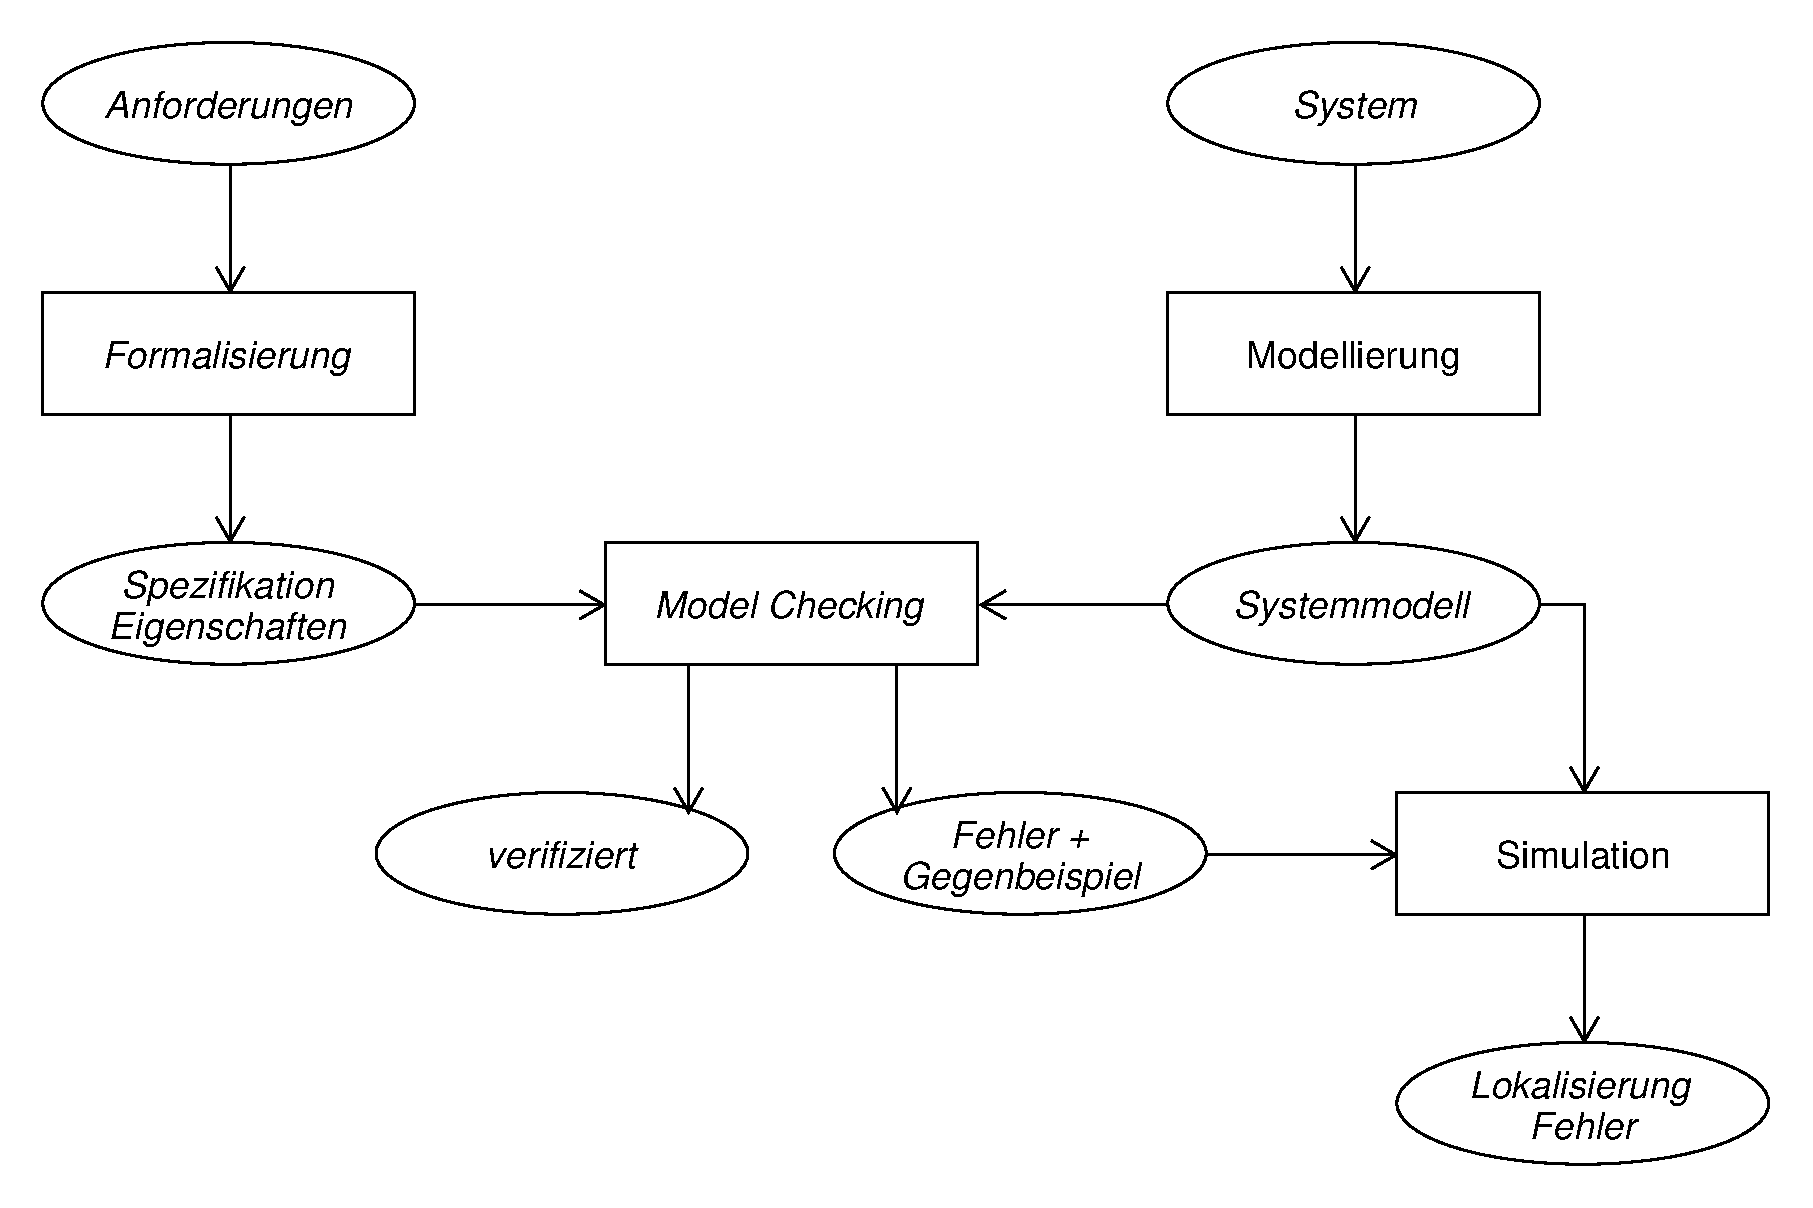
\includegraphics{./images/mcSchema.pdf}
	\caption[Schematischer Aufbau beim MC]{Schematischer Aufbau beim MC, nach \cite{Baier2008}}
	\label{fig:mcSchema}
\end{figure}

Ein \ac{MCr} nutzt, wie der Name schon sagt, ein Modell des Systems, um das System zu testen. Wie bei jeder anderen modellbasierten Technik ist daher die Qualität des \ac{MC} nur so gut wie das darauf zugrunde liegende Modell. Ein Modell kann auch als endlicher Automat angesehen werden, da ein Modell ebenfalls eine endliche Anzahl an möglichen Zuständen und dazugehörige Übergänge besitzt. Für jede Eigenschaft eines Zustandes muss zudem mithilfe einer sog. \emph{temporalen Logik}, also mathematisch bzw. formal, festgelegt werden, was gültige Werte dieser Eigenschaft sind. Die dazu benötigten Informationen werden aus den Anforderungen des Systems ermittelt und dem \ac{MCr} übergeben. So können später verschiedene Eigenschaften des gesamten Systems (\zB die formale Korrektheit, die Ausführbarkeit ohne Deadlocks oder die Einhaltung von Sicherheitsvorgaben) geprüft werden.

Zur Ausführung wird das gesamte Modell zunächst initialisiert und dann automatisch und systematisch vom \ac{MCr} auf Fehler und ungültige Zustände geprüft. In der Regel ist aber auch eine Ausführung als reine Simulation des Systems möglich, ohne explizit nach Fehlern zu suchen.

Wenn alle Zustände und deren Eigenschaften die Anforderungen erfüllen, erfüllt auch das Modell die Spezifikation. Wenn ein Zustand bzw. Eigenschaft die Anforderungen nicht erfüllt, prüft der \ac{MCr} anhand eines Gegenbeispiels den Ausführungspfad zum Fehler. Dadurch kann ermittelt werden, wo die Fehlerursache liegt. Einige der wesentlichen Fehlertypen und Ursachen sind:

\begin{description}
	\item[Modelling Error] Der Fehler liegt im Modell, welches korrigiert werden muss.
	\item[Design Error] Der Fehler liegt in den formellen oder informellen Anforderungen, dadurch muss das Modell und/oder die temporale Logik korrigiert werden.
	\item[Property Error] Der Fehler ist wirklich ein Fehler im System, welcher gefunden werden soll.
\end{description}

Möglich ist aber auch, dass die Ressourcen nicht ausreichen, um alle Zustände zu prüfen. In so einem Fall gibt es mehrere Möglichkeiten, damit umzugehen, \zB können Heuristiken oder Abstraktionen vom Modell genutzt werden \cite{Baier2008,Eberhardinger2016}.

\ac{MC} besitzt durch seine Charakteristik einige Vorteile, \uA \cite{Baier2008}:
\begin{itemize}
	\item \ac{MC} ist universell nutzbar, \zB für Software, Hardware oder eingebettete Systeme
	\item Partielle Verifikation ist möglich ohne das gesamte System testen zu müssen
	\item Vollständig automatisierbar und benötigt kaum Benutzerinteraktion oder hohe Expertise
\end{itemize}

Natürlich gibt es aber auch einige Nachteile, \uA \cite{Baier2008}:
\begin{itemize}
	\item Mit \ac{MC} wird nur ein Systemmodell und nicht das eigentliche System getestet, was weitere Fehler nicht ausschließt
	\item Hauptsächlich für steuerungsbasierte Anwendungen und nicht für datenbasierte Anwendungen geeignet
	\item Anzahl der möglichen Zustände kann zu hoch sein, um alle zu testen
\end{itemize}

Es gibt zahlreiche \ac{MC}-Frameworks, die bereits erwähnten \emph{LTSmin} und \emph{\sS} sind nur zwei davon.

\section{\sS}\label{sec:sSharp}

\sS ist ein am \isse der Universität Augsburg entwickeltes Testframework, das auch einen \ac{MC} beinhält. Da es in \cS entwickelt wurde und \cS auch zum Entwickeln von Modellen und dazugehörigen Testszenarien genutzt wird, können zahlreiche Features des .NET-Frameworks bzw. der Sprache \cS im Speziellen genutzt werden. \sS vereint dabei die Simulation, die Visualisierung, modellbasierte Tests sowie das \ac{MC} der Modelle \cite{Habermaier2015,Habermaier2016}. Dadurch können alle Schritte einer vollständigen Analyse inkl. Modellierung direkt im Visual Studio ausgeführt werden und somit auch alle Features der IDE und von .NET, wie \zB die Debugging-Werkzeuge, genutzt werden. Um den \ac{MCr} zu nutzen, hat \sS jedoch einige Einschränkungen, \uA sind Schleifen und Rekursionen nur eingeschränkt bzw. nicht möglich. Eine der größten Einschränkungen ist allerdings, dass während der Laufzeit keine neuen Objektinstanzen innerhalb des zu testenden Modells erzeugt werden können, sodass alle benötigten Instanzen bereits während der Initialisierung des Modells erzeugt werden müssen \cite{Habermaier2015}.

Um nun ein System testen zu können, muss dieses zunächst mithilfe von \cS-Klassen und -Instanzen modelliert werden. Die dafür verwendeten Modelle sind meist stark vereinfacht und bilden nur die wesentlichen Aspekte der realen Systeme ab. Für einen korrekten Test ist es jedoch wichtig, dass das Modell des Systems vergleichbar mit dem echten System ist.

\lstinputlisting[label=lst:ssExample,caption={Grundlegender Aufbau einer \sS-Komponente},float,style=cs]
{./listings/ssExample.cs}

\autoref{lst:ssExample} zeigt den typischen, grundlegenden Aufbau einer \sS-Komponente. Jede Komponente des Modells muss von \texttt{Component} erben, um als \sS-Komponente definiert zu sein. Jede Komponente kann nun temporäre (\texttt{TransientFault}) oder dauerhafte (\texttt{PermanentFault}) Komponentenfehler enthalten, welche zunächst innerhalb der Komponente als Felder definiert werden. Der Effekt eines Komponentenfehlers wird anschließend in der entsprechenden inneren Klasse definiert, welche von der Hauptklasse (hier \texttt{YarnNode}) erbt und mithilfe des Attributs \texttt{FaultEffect} dem dazugehörigen Komponentenfehler zugeordnet wird \cite{Habermaier2016}.

Um die Modelle zu testen, kommt in \sS die \ac{DCCA} zum Einsatz. Die \ac{DCCA} ermöglicht eine vollautomatisch und \ac{MC}-basierte Sicherheitsanalyse, wodurch selbstständig die Menge der aktivierten Komponentenfehler ermittelt wird, mit denen sich das Gesamtsystem nicht mehr rekonfigurieren kann und somit ausfällt. Je nach Konfiguration können dazu auch Heuristiken genutzt werden, welche die Analyse beschleunigen und genauer machen können \cite{Eberhardinger2016}. Dabei werden die verschiedenen aktivierten Komponentenfehler während der Analyse in tolerierbare und nicht-tolerierbare Fehler unterschieden. Tolerierbare Komponentenfehler werden dazu genutzt, die Grenzen der Selbstkonfiguration des Systems zu ermitteln. Dabei wird für jeden Systemzustand nach einer Rekonfiguration durch die \ac{DCCA} eine neue Fehlermenge ermittelt, mit der das System gerade noch so lauffähig ist. Das Auftreten eines tolerierbaren Komponentenfehler ist also gleichbedeutend mit einem einfachen Fehler im System, welcher die gesamte Funktionsweise des Systems nicht massiv einschränkt und es sich noch selbst rekonfigurieren kann. Sobald jedoch ein Fehler auftritt, durch den es dem System nicht mehr möglich ist, sich selbst zu rekonfigurieren, wurde ein nicht-tolerierbarer Fehler gefunden, durch den das System nicht mehr funktionsfähig ist \cite{Habermaier2015}.

    \chapter{Aufbau und Ablauf der Fallstudie}
\label{chap:caseStudy}

Im Rahmen dieser Masterarbeit soll nun mithilfe von Hadoop und der Selfbalancing"=Komponente eine Fallstudie durchgeführt werden, durch die ermittelt wird, unter welchen Umständen eine Testautomatisierung möglich ist.
\todo{Ergebnis zur Frage zur Testautomatistierung in Reflexion}
Hierfür werden mehrere Anforderungen an das durch den grundlegenden Versuchsaufbau definierte Modell gestellt.
Dieses Modell wird zur Realisierung der Tests mithilfe des \ac{ss}"=Frameworks als ein vereinfachtes Modell von Hadoop entwickelt und mit einem realen Cluster verbunden.

Teile der Beiträge und Inhalte dieses Kapitels wurden bereits in \cite{Eberhardinger2018} publiziert.

\section{Grundlegender Versuchsaufbau}
\label{sec:clusterSetup}

Neben den Anforderungen an Hadoop und das gesamte Testsystem muss auch der grundlegende Versuchsaufbau in dieser Fallstudie definiert werden.
Im Grunde wird, wie bereits in \autoref{chap:intro} erwähnt, Hadoop mithilfe des \ac{ss}"=Frameworks nachgebildet und dieses Modell mit einem realen Cluster verbunden.
\todo{dort erwähnen}
In diesem Cluster sollen anhand des Modells unterschiedliche Komponentenfehler injiziert und repariert werden, als auch unterschiedliche Benchmarks gestartet werden.
Hierbei soll nicht nur das Verhalten von Hadoop selbst analysiert werden, sondern auch das der von \citeauthor{zhang2016} entwickelten Selfbalancing"=Komponente.
Anhand dieses Verhaltens und dem des kompletten Testsystems soll schließlich ermittelt werden, ob eine Testautomatisierung in diesem Versuchsaufbau erfolgreich war.

Bei der Entwicklung des Modells liegt der Fokus auf dem grundlegenden Aufbau von \ac{YARN}.
Dazu gehören die Anwendungen und ihre Attempts, sowie zum Teil auch ihre Container.
Daneben muss das Modell auch die Nodes des Clusters und zum Ausführen der Benchmarks auch simulierte Clients enthalten.
Da bei den Tests auch Ausfälle von Nodes eine Rolle spielen, müssen hierfür entsprechende Komponentenfehler implementiert werden, die mithilfe von \ac{ss} aktiviert und deaktiviert werden können.

Da die Auswahl der ausgeführten Benchmarks eines jeden Clients nicht bei jedem Test manuell bestimmt werden soll, wird hierfür ein Transitionssystem verwendet.
Mithilfe dieses Transitionssystems, in dem die Wahrscheinlichkeiten von Wechseln zwischen zwei Anwendungen definiert sind, soll während der Ausführung eines Testfalls zufällig eine nachfolgende Anwendung ausgewählt werden.
%Da zum Testen des Clusters der \ac{ss}"=Simulator eingesetzt wird, hängt die Anzahl der Anwendungen primär von der Anzahl der ausgeführten Simulations"=Schritte ab.
%Ein weiterer Faktor zur Anzahl der Anwendungen ist die Anzahl an simulierten Clients, da auch getestet werden soll, wie sich das Cluster bei der Ausführung von mehreren parallel gestarteten Anwendungen verhält.

Die Verbindung zwischen dem Modell und dem realen Hadoop"=Cluster wird mithilfe eines dafür entwickelten Treibers durchgeführt.
Der Treiber ist dafür verantwortlich, Komponentenfehler und Anwendungen an das reale Cluster zu senden.
Zudem dient er dazu, um den Status des Clusters jederzeit ermitteln und an das Modell zur dortigen Speicherung übergeben zu können.
Er kann daher nicht nur aus der Verbindung zum Cluster selbst bestehen, sondern muss auch die Kommunikation zwischen Modell und Cluster sicherstellen und übermittelte Daten entsprechend umwandeln.

Zur Umsetzung des realen Clusters wird die von \citeauthor{zhang2016} entwickelte Plattform Hadoop"=Benchmark mit für diese Fallstudie entwickelten Szenarios genutzt.
Als Basis dient hierzu das bereits in der Plattform enthaltene Szenario mit der Nutzung der Selfbalancing"=Komponente.
Zudem soll auch mithilfe von Mutationstests, bei denen einer oder mehrere Mutanten in der Selfbalancing"=Komponente implementiert werden, das Testsystem geprüft werden.

Dieser Versuchsaufbau soll zudem mithilfe eines dafür entwickelten \emph{Oracles} geprüft werden.
Das Oracle dient zur Validierung der in \autoref{sec:requirements} definierten Anforderungen an das Cluster und das Testsystem.
Hierfür werden, sofern möglich, die Anforderungen als \emph{Constraints} im Modell implementiert und bei jedem Test automatisch geprüft.

Die Implementierung des eben beschriebenen Modells und Oracles ist im \autoref{chap:modell} beschrieben.
Die Auswahl der verwendeten Benchmarks und deren Implementierung mit dem Transitionssystem findet sich in \autoref{chap:benchmarks}.


\section{Anforderungen an das Cluster und Testsystem}
\label{sec:requirements}

Zur Überprüfung des Clusters und des Testssystems selbst werden hierfür jeweils mehrere Anforderungen gestellt.
Unterschieden wird hierbei zwischen funktionalen Anforderungen an das \gls{SuT} und Anforderungen an das Testsystem.
Während die funktionalen Anforderungen ausschließlich vom Hadoop"=Cluster als \gls{SuT} erfüllt werden müssen, müssen die Test"=Anforderungen vom gesamten Testsystem erfüllt werden.

Mithilfe der im Folgenden definierten Anforderungen soll bereits automatisiert geprüft werden, inwieweit eine Testautomatisierung möglich ist.
Hierfür werden die Anforderungen, sofern möglich, in Form von Constraints ebenfalls im Modell implementiert und während der Ausführung durch das Oracle validiert.

\subsection{Funktionale Anforderungen an das Cluster}
\label{subsec:functionalRequirements}

Obwohl in dieser Masterarbeit der Fokus auf Testautomatisierung und Validieren eines Testsystems liegt, müssen auch die funktionalen Anforderungen an das \gls{SuT}, also das Hadoop"=Cluster selbst, berücksichtigt werden.
Da im Rahmen der Publikation \cite{Eberhardinger2018} ebenfalls der in \cref{sec:clusterSetup} beschriebene, und in dieser Fallstudie genutzte Versuchsaufbau genutzt wurde, wurden im Rahmen dieser Fallstudie auch funktionale Anforderungen an das Cluster selbst durch das Oracle geprüft.
Dies betrifft konkret folgende Anforderungen an das \gls{SuT} \cite{Eberhardinger2018}:

\begin{enumerate}
    \item Ein Task wird vollständig ausgeführt, sofern er nicht abgebrochen wird
    \item Kein Task oder Anwendung wird an inaktive, defekte oder nicht verbundene Nodes gesendet
    \item Die Konfiguration wird aktualisiert, sobald eine entsprechende Regel erfüllt ist
    \item Defekte oder Verbindungsabbrüche werden erkannt
\end{enumerate}

\subsection{Anforderungen an das Testsystem}
\label{subsec:testRequirements}

Neben den funktionalen Anforderungen, gibt es weitere Anforderungen an das gesamte Testsystem.
Diese Anforderungen betreffen das Hadoop"=Cluster, die Selfbalancing"=Komponente, das entwickelte \gls{ss}"=Modell sowie den Treiber zur Kommunikation zwischen Modell und Cluster.
Konkret sind dies folgende Anforderungen an das Testsystem:

\begin{enumerate}
    \item Der \gls{MARP}"=Wert ändert sich, basierend auf den derzeit ausgeführten Anwendungen
    \item Der jeweils aktuelle Status des Clusters wird erkannt und im Modell gespeichert
    \item Defekte Nodes und Verbindungsabbrüche werden erkannt
    \item Im Modell implementierte Komponentenfehler werden im realen Cluster injiziert und repariert
    \item Wenn alle Nodes defekt sind, wird erkannt, dass sich das Cluster nicht mehr rekonfigurieren kann
    \item Ein Test kann vollautomatisch ausgeführt werden
    \item Das Cluster kann ohne Auswirkungen auf seine Funktionsweise auf einem oder mehreren Hosts ausgeführt werden
    \item Es können mehrere Benchmark"=Anwendungen gleichzeitig gestartet und ausgeführt werden
    \item Tests und Testfälle können zeitlich unabhängig und mehrmals ausgeführt werden
\end{enumerate}

Die funktionalen Anforderungen dienen zudem ebenfalls als Anforderungen an das Testsystem und erweitern somit die hier genannten Anforderungen.

Eine Besonderheit bildet die fünfte Anforderung, wonach erkannt werden muss, dass im Cluster keine weitere Rekonfiguration möglich ist.
Wird diese Anforderung verletzt, soll der ausgeführte Test abgebrochen werden, während bei den anderen, auch den funktionalen, Anforderungen dies nur durch das Oracle vermerkt, die Ausführung aber nicht weiter beeinträchtigt werden soll.


\section{Anforderungen an das Testsystem}
\label{sec:evaluationPlan}

Um das Testsystem zu validieren, wurde zunächst ein Evaluationsplan aufgestellt.
In diesem ist festgehalten, was getestet wird, wie die Testfälle aussehen und wie die bei der Ausführung gewonnen Daten organisiert werden.

\subsection{Behauptungen und Variablen}
\label{sec:predictions}

% Was für Behauptungen wurden aufgestellt
\begin{enumerate}
    \setcounter{enumi}{4}
    \item Der jeweils aktuelle Status des Clusters wird erkannt und im Modell gespeichert
    \item Defekte Nodes und Verbindungsabbrüche werden erkannt
    \item Im Modell implementierte Komponentenfehler werden im realen Cluster injiziert und repariert
    \item Wenn alle Nodes defekt sind, wird erkannt, dass sich das Cluster nicht mehr rekonfigurieren kann
    \item Ein Test kann vollautomatisch ausgeführt werden
    \item Das Cluster kann ohne Auswirkungen auf die Funktionsweise auf einem oder beiden Hosts ausgeführt werden
    \item Es können mehrere Benchmark"=Anwendungen gleichzeitig gestartet und ausgeführt werden
    \item Ein Testfall kann zeitlich unabhängig und mehrmals ausgeführt werden
\end{enumerate}

% Was für Variablen wurden dadurch ermittelt

\subsection{Generierung der Testfälle}
\label{sec:testcaseGeneration}

Die Generierung der Testfälle hängt von mehreren Faktoren ab.
Zum einen ist ein Testfall abhängig von der Größe des Clusters, also ob das Cluster auf einem oder beiden Hosts ausgeführt wird und aus wie vielen Nodes das Cluster besteht.
Relevant zur Unterscheidung von Testfällen sind aber auch die ausgeführten Anwendungen.
Da die Auswahl der ausgeführten Anwendungen nicht manuell bestimmt werden soll, wird hierfür ein Transitionssystem verwendet.
Mithilfe dieses Transitionssystems, in dem die Wahrscheinlichkeiten von Wechsel zwischen zwei Anwendungen definiert sind, soll während der Ausführung eines Testfalls zufällig eine nachfolgende Anwendung ausgewählt werden.
Da zum Testen des Clusters der \ac{ss}"=Simulator eingesetzt wird, hängt die Anzahl der Anwendungen primär von der Anzahl der ausgeführten Simulations"=Schritte ab.
Ein weiterer Faktor zur Anzahl der Anwendungen ist die Anzahl an simulierten Clients, da auch getestet werden soll, wie sich das Cluster bei der Ausführung von mehreren parallel gestarteten Anwendungen verhält.
Die zu injizierenden Komponentenfehler, mit denen defekte Nodes und Verbindungsausfälle simuliert werden, werden ebenfalls zufallsbasiert ausgewählt.
Dies gilt auch für das Deaktivieren der Komponentenfehlern.

Die Auswahl der nachfolgenden Anwendungen und die Entscheidung über die Aktivierung und Deaktivierung der Komponentenfehlern wird daher mithilfe eines Zufallsgenerators realisiert.
Hierbei soll jedoch kein echter Zufallsgenerator zum Einsatz kommen, sondern ein Pseudo"=Zufallsgenerator.
Da ein Pseudo"=Zufallsgenerator seine Werte mithilfe eines Start"=\emph{Seeds} auswählt, besteht somit die Möglichkeit durch die Verwendung eines bestimmten Seeds, einen Testfall jederzeit wiederholen zu können.
Zur Auswahl der ersten Testfälle werden daher zeitbasierte Seeds verwendet.
Diese Seeds werden bei der Ausführung notiert und für andere Testfälle verwendet, bei denen andere Punkte der Konfiguration wie \zB die Größe des Clusters, abgeändert werden.
Dadurch ist es möglich, die Auswirkungen einzelner Parameter zu testen und zu evaluieren.
\todo{Wo wird Seed wie genutzt? am besten in implementierung davon!}

\subsection{Organisation und Ausgabe der Daten}
\label{sec:dataOrganisation}

Damit die bei der Ausführung gewonnenen Daten auch zur Evaluation genutzt werden können, wurde hierzu festgelegt, welche Daten während der Ausführung ausgegeben werden.
Alle relevante Daten werden hierzu während der Ausführung der Testfälle in einer Log"=Datei gespeichert.
Zur Unterscheidung von einzelnen Ausführungen werden die Daten klar strukturiert.
Neben den im folgenden beschriebenen Daten werden zudem alle Ein- und Ausgabedaten der SSH"=Verbindungen zwischen \ac{ss} und dem Cluster (vgl. \autoref{sec:aufbauCluster}) in einem eigenen Log gespeichert.

Beim Start der Simulation werden zunächst einige generelle Daten ausgegeben:

\begin{itemize}
    \item Basis"=Seed für die Zufallsgeneratoren
    \item Mindestdauer für einen Simulations"=Schritt
    \item Anzahl der ausgeführten Simulations"=Schritte
    \item Wahrscheinlichkeiten für Aktivierung und Deaktivierung der Komponentenfehler
    \item Angabe, ob vorab generierte Eingabedaten genutzt werden oder diese während der Ausführung eines Testfalls generiert werden
    \item Anzahl genutzter Hosts und Nodes
    \item Pfade verwendeter Scripte auf den Hosts (vgl. \autoref{sec:aufbauCluster})
    \item Bei der Nutzung der REST"=API verwendete URL des Controllers
    \item Auszuführende Benchmarks    
\end{itemize}

Die Ausgabe der Daten der YARN"=Komponenten wird bei jedem Simulations"=Schritt durchgeführt, damit das Verhalten des Clusters berücksichtigt werden kann.
Ausgegeben werde hierbei:

\begin{itemize}
    \item Für jeden Node:
    \begin{itemize}
        \item ID bzw. Name des Nodes
        \item Aktueller Status
        \item Informationen zur Fehleraktivierung
        \item Anzahl ausgeführter Container auf dem Node
        \item Angaben zur Speicherauslastung
        \item Angaben zur CPU"=Auslastung
    \end{itemize}
    
    \item Für jeden Client:
    \begin{itemize}
        \item ID bzw. Name des Clints
        \item Aktuell ausgeführter Benchmark
        \item ID der aktuell ausgeführten Anwendung auf dem Cluster
    \end{itemize}

    \item Für jede Anwendung:
    \begin{itemize}
        \item ID der Anwendung
        \item Bezeichnung der Anwendung
        \item Aktueller und finaler Status der Anwendung
        \item ID bzw. Name des Nodes, auf dem der \ac{AppMstr} ausgeführt wird
    \end{itemize}

    \item Für jeden Attempt:
    \begin{itemize}
        \item ID des Attempts
        \item Aktueller Status des Attempts
        \item ID des \ac{AppMstr}"=Containers
        \item ID bzw. Name des Nodes, auf dem der \ac{AppMstr} ausgeführt wird
    \end{itemize}

    \item Für jeden Container:
    \begin{itemize}
        \item ID des Containers
        \item ID bzw. Name des auszuführenden Nodes
        \item Aktueller Status des Containers
    \end{itemize}
\end{itemize}

Die Details zur Implementierung und dem Ausgabeformat sind in \autoref{sec:simulationStepOutput} erläutert.


    \chapter{Aufbau des Modells}\label{chap:model}

\section{Grundlegende Architektur}\label{sec:architecture}

\begin{wrapfigure}{r}{0.5\columnwidth}
	\centering
	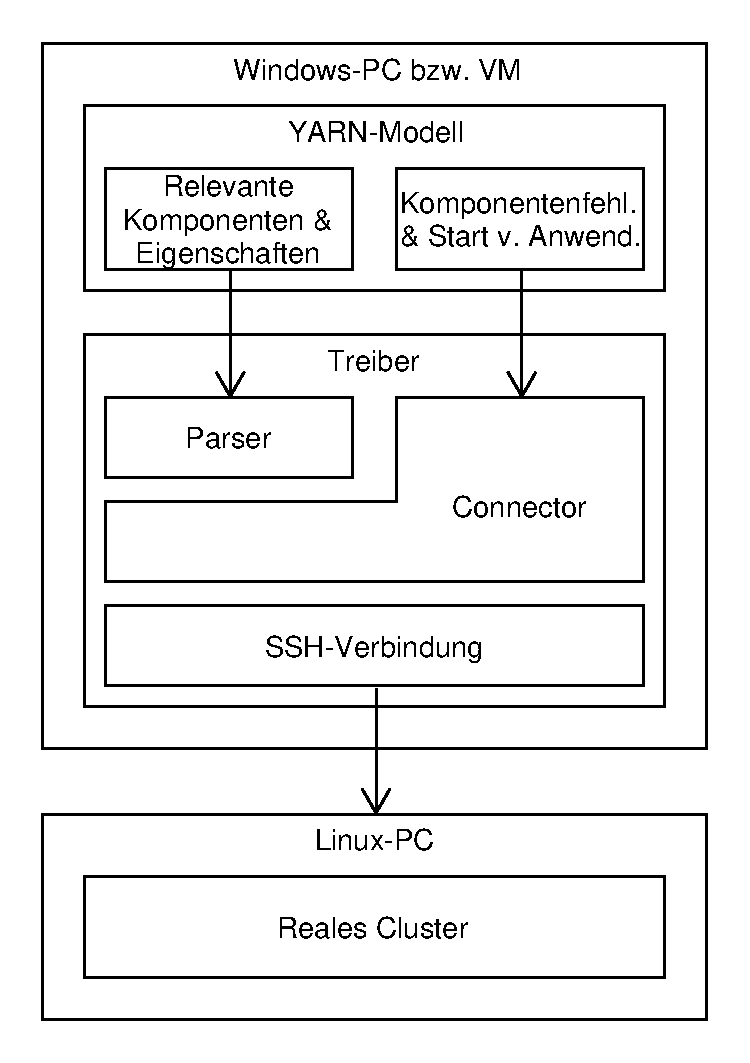
\includegraphics[width=0.5\columnwidth]{./images/modelArchitecture.pdf}
	\caption{Grundlegende Architektur des Gesamtmodells}
	\label{fig:modelArchitecture}
\end{wrapfigure}

Die grundlegende Architektur des gesamten Aufbaus besteht aus den drei in \autoref{fig:modelArchitecture} zu sehenden Schichten. Die oberste Schicht bildet dabei das \sS-Modell von Hadoop YARN, welches die wesentlichen YARN-Komponenten und dessen Komponentenfehler abbildet. Das reale Pendant dazu bildet das reale Cluster als unterste Schicht. Die Verbindung zwischen dem Modell und dem realen Cluster bildet der Treiber als eigenständige Schicht, bestehend aus den Kernkomponenten Parser, Connector und der eigentlichen SSH-Verbindung zum realen Cluster. Da \sS auf dem .NET-Framework aufbaut, ist für den \sS-MC entsprechend ein Windows dafür nötig, während das reale Cluster auf einem eigenen Linux-PC ausgeführt wird, weshalb als Konsequenz zur Kommunikation zwischen Modell und Cluster eine SSH-Verbindung nötig ist.

\section{\sS-Modell}\label{sec:sSharpModel}



\section{Reales Hadoop-System}\label{sec:realHadoop}



\section{SSH-Treiber}\label{sec:sshDriver}

Im Einführungstext zu diesem Kaptiel wurde bereits auf den grundlegenden Aufbau des Treibers eingegangen. Der SSH-Treiber besteht aus den drei einzelnen Komponenten Parser, Connector und SSH-Verbindung, von denen die ersten beiden mithilfe von Interfaces im YARN-Modell eingebunden sind. Dadurch ist es möglich, unterschiedliche Parser bzw. auch Verbindungen für unterschiedliche Komponenten zu nutzen.

Der Parser selbst besteht neben dem eigentlichen Parser zudem aus Datenhaltungs-Klassen für die relevanten YARN-Komponenten. Sie dienen dazu, die geparsten Rohdaten von Hadoop an das \sS-Modell zu übergeben und sind daher ebenfalls mithilfe von entsprechenden Interfaces im Modell eingebunden. Die Implementierungen der Klassen selbst sind außerdem so aufgebaut, dass sie für beide hier implementierten Parser genutzt werden können.

\subsection{Kommandozeilen-Parser}\label{sec:cmdParser}

% Was gibt Hadoop aus
Hadoop besitzt zur Steuerung einige Kommandozeilen-Befehle, mit denen \uA auch die Daten der YARN-Komponenten ausgelesen werden können. Die Daten werden mithilfe der Befehle immer vom \ac{RM} und, sofern gestartet, vom Timeline-Server ermittelt und ausgegeben. Ausgegeben werden können \uA die Daten zu:

\begin{description}[noitemsep]
    \item[Anwendungen] als nach dem Status gefilterte Liste oder der Report einer Anwendung
    \item[Ausführungen] als Liste aller Ausführungen einer Anwendung oder der Report einer Ausführung
    \item[Container] als Liste aller Container einer Ausführung oder der Report eines Containers
    \item[Nodes] als Liste aller Nodes oder der Report eines Nodes
\end{description}

Einige Beispiele für die dafür notwendigen Befehle sowie deren mögliche Ausgaben sind in \autoref{app:hadoopCmds} zu finden.

% Wie wurde der Parser aufgebaut

\subsection{REST-API-Parser}\label{sec:restParser}

% Was gibt Hadoop aus
% Wie wurde der Parser aufgebaut

\subsection{Connector}\label{sec:Connector}

% Wie wird die Verbindung abstrahiert

\subsection{SSH-Verbindung}\label{sec:sshConnection}

% Wie funktioniert die Verbindung selbst

    \chapter{Implementierung der Benchmarks}
\label{ch:benchmarks}

Neben dem \gls{YARN}"=Modell selbst sind auch die während der Testausführung genutzten \glspl{Anwendung} ein wichtiger Bestandteil des gesamten Testmodells.
Da Hadoop selbst sowie die Plattform Hadoop"=Benchmark bereits einige \glspl{Anwendung} und Benchmarks enthalten, konnten diese auch im Rahmen dieser Fallstudie genutzt werden.
Dazu wurde eine Auswahl an \glspl{Anwendung} in einer Markow"=Kette miteinander verbunden, mit dem die Ausführungsreihenfolge der einzelnen \glspl{Anwendung} basierend auf Wahrscheinlichkeiten bestimmt wird.
Verwaltet werden die implementierten Benchmarks mithilfe des Benchmark"=Controllers.

Da für die in \cite{Eberhardinger2018} durchgeführte Fallstudie das für diese Fallstudie entwickelte Testmodell genutzt wurde, enthält es auch das hierfür entwickelte Transitionssystem.
Daher wurden Teile der Beiträge dieses Kapitels dort bereits publiziert.

\section{Übersicht möglicher Anwendungen}\label{sec:appOverview}

Hadoop-Benchmark enthält bereits die Möglichkeit, unterschiedliche Benchmarks zu starten. Wie in \autoref{sec:hadoopBenchmark} erwähnt, sind folgende Benchmarks in der Plattform integriert:

\begin{itemize}
    \item Hadoop Mapreduce Examples
    \item Intel HiBench
    \item \ac{SWIM}
\end{itemize}

Jeder Benchmark enthält zum Starten ein jeweiliges Start"=Script, mit dem ein neuer Docker"=Container auf der Controller"=VM gestartet wird, mit dem der Benchmark auf dem Cluster gestartet wird. Dass dafür ein eigener Docker-Container genutzt wird liegt daran, dass es in Docker"=Umgebungen \emph{best practice} ist, einen Docker"=Container für nur einen Einsatzzweck zu erstellen und zu nutzen. Die Hauptgründe dafür sind, dass dadurch die Skalierbarkeit erhöht und die Wiederverwendbarkeit gesteigert werden \cite{DockerBestPractice}. Daher wurden auch die Startscripte für die Benchmarks so angepasst, dass die jeweiligen Benchmarks mehrfach gestartet werden können.

Die \textbf{Hadoop Mapreduce Examples} sind unterschiedliche und meist voneinander unabhängige Anwendungen, die beispielhaft für die meisten Anwendungsfällen in einem produktiv genutzten Cluster sind. Die Examples sind Teil von Hadoop und daher bei jeder Hadoop"=Installation enthalten. Einige der Anwendungen der Examples sind:

\begin{itemize}
    \item Generatoren für Text und Binärdaten, \zB \acl{rtw}
    \item Analysieren von Daten, \zB \acl{wc}
    \item Sortieren von Daten, \zB \acl{sort}
    \item Ausführen von komplexen Berechnungen, \zB \emph{Bailey-Borwein-Plouffe-Formel} zur Berechnung einzelner Stellen von $\pi$
\end{itemize}

\textbf{Intel HiBench} ist eine Benchmark-Suite mit \emph{Workloads} zu verschiedenen Anwendungszwecken mit jeweils unterschiedlichen einzelnen Anwendungen. Da in Hadoop"=Benchmark noch die HiBench"=Version \mbox{2.2} verwendet wird, wurde der Docker"=Container von HiBench zunächst auf Version 7 aktualisiert, die einige neuen Workloads und Anwendungen enthält. HiBench enthält damit folgende Workloads mit einer unterschiedlichen Anzahl an möglichen Anwendungen:

\begin{itemize}
    \item Micro"=Benchmarks (basieret auf den Mapreduce"=Examples und den Jobclient"=Tests)
    \item Maschinelles Lernen
    \item SQL/Datenbanken
    \item Websuche
    \item Graphen
    \item Streaming
\end{itemize}

\textbf{\ac{SWIM}} ist eine Benchmark-Suite, die aus 50 verschiedenen Workloads besteht. Das besondere dabei ist, dass die dabei verwendeten Mapreduce"=Jobs anhand mehrerer tausend Jobs erstellt wurden und im Vergleich zu anderen Benchmarks eine größere Vielfalt an Anwendungen und somit ein größerer Testumfang gewährleistet wird \cite{SwimWikiHome}. Bei der Ausführung auf dem in dieser Arbeit verwendete Cluster wurden jedoch nicht alle Workloads fehlerfrei ausgeführt. Zudem wird in \cite{InriaTutorial} explizit erwähnt, dass es bei der Ausführung auf einem Cluster auf einem einzelnen PC bzw. Laptop Probleme geben kann. Zudem ist SWIM für Benchmarks eines Clusters mit mehreren physischen Nodes ausgelegt ist und daher würde die Ausführung in dieser Fallstudie extrem viel Zeit benötigten. Daher wurde die Nutzung des SWIM-Benchmarks nicht weiter verfolgt.

Ebenfalls im Installationsumfang von Hadoop enthalten sind die sog. \textbf{Jobclient"=Tests}. Hauptbestandteil dieser Tests sind vor allem weitere Benchmarks, welche das gesamte Cluster oder einzelne Nodes testen, wobei die meisten Anwendungen das \ac{HDFS} betreffen. Da die Jobclient-Tests kein Teil von Hadoop"=Benchmark sind, wurde zur Ausführung der Jobclient"=Test zunächst ein eigenes Start"=Script analog zur Ausführung der Mapreduce"=Examples erstellt, damit hierfür ebenfalls ein eigener Docker"=Container gestartet wird. Die Jobclient"=Tests enthalten \uA folgende Arten an Anwendungen:

\begin{itemize}
    \item \ac{HDFS}"=Systemtests, \zB \texttt{SilveTest}
    \item Reine Lastgeneratoren, \zB \texttt{NNloadGenerator}
    \item Eingabe/Ausgabe"=Durchsatz"=Tests, \zB \texttt{TestDFSIO}
    \item Dummy"=Anwendungen \texttt{sleep} (blockiert Ressourcen, führt aber nichts aus) und \texttt{fail} (Anwendung schlägt immer fehl)
\end{itemize}

\section{Auswahl der verwendeten Anwendungen}
\label{sec:appSelection}

Damit die Fallstudie die Realität abbilden kann, wurden von allen verfügbaren Anwendungen einige ausgewählt und in ein Transitionssystem in Form einer Markow"=Kette überführt.
Diese Kette definiert die Ausführungsreihenfolge zwischen den einzelnen Anwendungen.
Eine zufallsbasierte Markow"=Kette wurde aus dem Grund verwendet, dass auch in der Realität Anwendungen nicht immer in der gleichen Reihenfolge ausgeführt werden und daher auch in der Fallstudie eine unterschiedliche Ausführungsreihenfolge der Anwendungen gewährleistet werden soll.
Mithilfe der Festlegung eines bestimmten Seeds für den in der Fallstudie benötigten Pseudo"=Zufallsgenerator besteht bei Bedarf dennoch die Möglichkeit, einen Test mit den gleichen Anwendungen wiederholen zu können.

Einige der in \cref{sec:appOverview} erwähnten Mapreduce Examples werden häufig als Benchmark verwendet.
Einige Beispiele dafür sind die Anwendungen \acl{so} und \texttt{grep}, die bereits im Referenzpapier des \ac{MR}"=Frameworks zum Testen genutzt wurden \cite{Dean2004}.
Zum Testen des \ac{HDFS} dient in \cite{Shvachko2010} der DFSIO"=Benchmark, um den Durchsatz beim Lesen und Schreiben einer großen Datenmenge auf dem \ac{HDFS} zu messen.
\acl{tsr} ist ebenfalls ein weit verbreiteter Benchmark, der die Hadoop"=Implementierung der standardisierten \emph{Sort Benchmarks}\footnote{\url{https://sortbenchmark.org/}} darstellt \cite{Graves2013}.
Ebenfalls als guter Benchmark dient die Anwendung \acl{wc}, mit der ein großer Datensatz stark verkleinert bzw. zusammengefasst wird und dient daher als gute Repräsentation für Anwendungsarten, bei denen Daten extrahiert werden \cite{Huang2010,Chen2012}.

Da in dieser Fallstudie ein realistisches Abbild der ausgeführten Anwendungen ausgeführt werden soll, ist es nicht sehr hilfreich, die einzelnen Übergangswahrscheinlichkeiten im Transitionssystem anzugleichen oder rein zufällig zu verteilen.
Einen realistischen Einblick, welche Anwendungs- und Datentypen in produktiv genutzten Hadoop"=Clustern genutzt werden, geben \uA \cite{Chen2012} und \cite{HadoopDataTypes}.
Auffällig ist hierbei, dass die meisten Anwendungen in einem Hadoop"=Cluster innerhalb weniger Sekunden oder Minuten abgeschlossen sind und/oder Datensätze im Größenbereich von wenigen Kilobyte bis hin zu wenigen Megabyte verarbeiten.
Zu einem ähnlichen Ergebnis kamen auch \citeauthor{Ren2013} in \cite{Ren2013} und folgerten daher, dass für kleine Jobs evtl. einfachere Frameworks abseits von Hadoop besser geeignet wären.
Die Autoren der Studie in \cite{HadoopDataTypes} bezeichneten Hadoop aufgrund ihrer Ergebnisse als \enquote{potentielle Technologie zum Verarbeiten aller Arten von Daten}, stellten aber eine ähnliche Vermutung an wie \citeauthor{Ren2013}, dass Hadoop primär Daten nutze, die auch mit \enquote{traditionellen Plattformen} verarbeiten werden könnten.

Basierend auf den Ergebnissen der Studien in \cite{Huang2010,Chen2012,HadoopDataTypes,Ren2013} und der in den Publikationen \cite{Shvachko2010,Dean2004,Graves2013} verwendeten Benchmark"=Anwendungen, wurden folgende Anwendungen der Mapreduce Examples und Jobclient"=Tests in das Transitionssystem übernommen:

\begin{itemize}
    \item Generieren von Eingabedaten für andere Anwendungen:
    \begin{itemize}
        \item Textdateien:
        \begin{itemize}
            \item \ac{rtw}: Generierung von zufälligen Zeichenfolgen
            \item \ac{dfw}: Schreiben einer großen Datenmenge auf dem \ac{HDFS}
        \end{itemize}
        \item Binärdateien:
        \begin{itemize}
            \item \ac{rw}: Generierung von zufälligen Binärdaten
            \item \ac{tg}: Generierung der Eingabedaten für den \acl{tsr}"=Benchmark
       \end{itemize}
    \end{itemize}

    \item Verarbeitung von Eingabedaten:
    \begin{itemize}
        \item Auslesen bzw. Zusammenfassen:
        \begin{itemize}
            \item \ac{wc}: Auslesen einer Textdatei und Ermitteln der Anzahl der darin enthaltenen Wörter
            \item \ac{dfr}: Auslesen einer großen Datenmenge auf dem \ac{HDFS}
        \end{itemize}
        \item Transformieren:
        \begin{itemize}
            \item \ac{so}: Sortieren von Daten, wird in dieser Fallstudie zum Sortieren von Textdaten genutzt
            \item \ac{tsr}: Sortieren von großen Binärdatenmengen
        \end{itemize}
        \item Validierung der Transformationen:
        \begin{itemize}
            \item \ac{tms}: Validierung der von \acl{so} transformierten Daten
            \item \ac{tvl}: Validierung der vom \acl{tsr} sortierten Binärdaten
        \end{itemize}
    \end{itemize}

    \item Ausführen von Berechnungen:\todo{evtl. noch literatur dazu finden}
    \begin{itemize}
        \item \acl{pi}\acused{pi}: Ausführung der Quasi"=Monte"=Carlo"=Methode zur einfachen Berechnung von $\pi$
        \item \ac{pt}: Berechnung von Pentomino"=Problemen
    \end{itemize}

    \item Dummy"=Anwendungen:
    \begin{itemize}
        \item  \ac{sl}: Blockieren von Ressourcen
        \item  \ac{fl}: Fehlschlagen einer Anwendung
    \end{itemize}
\end{itemize}

Der Grund für die Berücksichtigung von mehreren gleichen bzw. ähnlichen Anwendungen für einige Kategorien liegt darin, dass die unterschiedlichen Anwendungen eine unterschiedliche Ausführungsdauer bzw. Datenrepräsentation (Text und Binär) repräsentieren.
So stehen die beiden \texttt{TestDFSIO}"=Varianten für eine umfangreichere Datennutzung, während die jeweils anderen Anwendungen einen kleineren Umfang repräsentieren.
Ähnlich verhält es sich bei den beiden Berechnungs"=Anwendungen, bei denen die \acl{pt}"=Anwendung die deutlich umfangreicheren Berechnungen durchführt.
\texttt{TestDFSIO} enthält zudem die Möglichkeit, Daten zu generieren und zu lesen, weshalb dieser Benchmark in zwei Kategorien als Anwendung genutzt wird.

Eine Besonderheit bilden die beiden Dummy"=Anwendungen.
Beide werden in dieser Fallstudie dafür genutzt, um zu simulieren, wenn auf dem Cluster \zB derzeit nichts ausgeführt wird, oder ein Fehler während der Ausführung einer Anwendung auftritt.
Daher können beide Anwendungen unabhängig von der derzeit ausgeführten Anwendung als nachfolgende Anwendung ausgewählt werden.
Als nachfolgende Anwendungen für die Dummy"=Anwendungen wurden nur Anwendungen definiert, die ihrerseits keine Eingabedaten benötigten bzw. diese für andere Anwendungen generieren:

\begin{itemize}
    \item \acl{dfw}
    \item \acl{rtw}
    \item \acl{tg}
    \item \acl{rw}
    \item \acl{pi}
    \item \acl{pt}
\end{itemize}

\begin{table}
    \resizebox{\linewidth}{!}{\begin{tabu}{l|[1.5pt]c|c|c|c|c|c|c|c|c|c|c|c|c|c}
    	                   & \textit{\acs{dfw}} & \textit{\acs{rtw}} & \textit{\acs{tg}} & \textit{\acs{dfr}} & \textit{\acs{wc}} & \textit{\acs{rw}} & \textit{\acs{so}} & \textit{\acs{tsr}} & \textit{\acs{pi}} & \textit{\acs{pt}} & \textit{\acs{tms}} & \textit{\acs{tvl}} & \textit{\acs{sl}} & \textit{\acs{fl}} \\ \tabucline[1.5pt]{-}
    	\textit{\acs{dfw}} &        .600        &        .073        &         0         &        .145        &         0         &         0         &         0         &         0          &       .073        &       .073        &         0          &         0          &       .018        &       .018        \\ \hline
    	\textit{\acs{rtw}} &        .036        &        .600        &         0         &         0          &       .145        &       .036        &       .109        &         0          &       .036        &         0         &         0          &         0          &       .019        &       .019        \\ \hline
    	\textit{\acs{tg}}  &         0          &        .036        &       .600        &         0          &         0         &         0         &         0         &        .255        &         0         &       .073        &         0          &         0          &       .018        &       .018        \\ \hline
    	\textit{\acs{dfr}} &         0          &        .073        &         0         &        .600        &         0         &       .036        &         0         &         0          &       .145        &       .109        &         0          &         0          &       .018        &       .019        \\ \hline
    	\textit{\acs{wc}}  &        .073        &        .109        &         0         &         0          &       .600        &         0         &       .073        &         0          &       .073        &       .036        &         0          &         0          &       .018        &       .018        \\ \hline
    	\textit{\acs{rw}}  &         0          &        .073        &       .073        &         0          &         0         &       .600        &         0         &         0          &       .109        &       .109        &         0          &         0          &       .018        &       .018        \\ \hline
    	\textit{\acs{so}}  &         0          &        .073        &       .036        &         0          &       .073        &       .036        &       .600        &         0          &       .073        &         0         &        .073        &         0          &       .018        &       .018        \\ \hline
    	\textit{\acs{tsr}} &         0          &         0          &         0         &         0          &         0         &         0         &         0         &        .600        &       .109        &       .073        &         0          &        .182        &       .018        &       .018        \\ \hline
    	\textit{\acs{pi}}  &        .145        &        .109        &         0         &         0          &         0         &         0         &         0         &         0          &       .600        &       .109        &         0          &         0          &       .018        &       .019        \\ \hline
    	\textit{\acs{pt}}  &        .109        &        .109        &         0         &         0          &         0         &       .073        &         0         &         0          &       .073        &       .600        &         0          &         0          &       .018        &       .018        \\ \hline
    	\textit{\acs{tms}} &         0          &        .145        &         0         &         0          &         0         &       .073        &         0         &         0          &       .036        &       .109        &        .600        &         0          &       .018        &       .019        \\ \hline
    	\textit{\acs{tvl}} &        .073        &        .109        &         0         &         0          &         0         &         0         &         0         &         0          &       .109        &       .073        &         0          &        .600        &       .018        &       .018        \\ \hline
    	\textit{\acs{sl}}  &        .167        &        .167        &       .167        &         0          &         0         &       .167        &         0         &         0          &       .167        &       .167        &         0          &         0          &         0         &         0         \\ \hline
    	\textit{\acs{fl}}  &        .167        &        .167        &       .167        &         0          &         0         &       .167        &         0         &         0          &       .167        &       .167        &         0          &         0          &         0         &         0
    \end{tabu}}
    \caption
    {Verwendete Markov"=Kette für die Anwendungs"=Übergänge in Tabellenform.}
    \label{tab:transMatrix}
\end{table}

Für die in \cref{tab:transMatrix} dargestellte Markow"=Kette der Übergänge zwischen den Anwendungen wurde neben den Ergebnissen aus den Studien zudem berücksichtigt, welche Anwendungen bestimmte Eingabedaten benötigen.
Dadurch wird sichergestellt, dass die für einige Anwendungen benötigten Eingabedaten immer vorhanden sind, da diese ebenfalls im Rahmen der Ausführung der Benchmarks generiert werden.
Anwendungen ohne Eingabedaten können dagegen fast jederzeit ausgeführt werden.


\section{Implementierung der Anwendungen im Modell}
\label{sec:appImplementation}

Die Verwaltung der auszuführenden Benchmarks wurde komplett vom restlichen YARN"=Modell getrennt.
Verbunden sind beide durch die Eigenschaft \texttt{Client.BenchController}, das den vom Client verwendeten \texttt{BenchmarkController} enthält, der zur Verwaltung der auszuführenden Anwendung dient.
Der Controller besteht aus zwei wesentlichen Teilen, einem statischen und einem dynamischen.

Der \textbf{statische Teil} des Controllers definiert die möglichen Anwendungen sowie das im Abschnitt zuvor definierte und in \cref{tab:transMatrix} dargestellte Transitionssystem.
Die einzelnen Anwendungen werden mithilfe der Klasse \texttt{Benchmark} repräsentiert, in der die benötigten Informationen wie \zB der Befehl zum Starten der Anwendung definiert werden.
Da mehrere Clients unabhängig voneinander agieren können müssen, erhält jeder Client zudem ein eigenes Unterverzeichnis im \ac{HDFS}, in dem sich die Ein- und Ausgabeverzeichnisse für die von ihm gestarteten Anwendungen befinden.
Das muss auch bei der Definition der Startbefehle der Anwendungen berücksichtigt werden, weshalb in \cref{lst:benchmarkDefinition} entsprechende Platzhalter vorhanden sind.
Aus diesem Grund muss vor dem Start der Anwendung mithilfe der Methode \texttt{GetStartCmd()} der Startbefehl generiert werden, indem der zu startende Client das in \texttt{Client.ClientDir} gespeicherte Client"=Basisverzeichnis übergibt.
Da einige Anwendungen zudem voraussetzen, dass das genutzte Ausgabe"=Verzeichnis noch nicht im \ac{HDFS} existiert, muss das Verzeichnis vor dem Anwendungsstart gelöscht werden.

Jede Anwendung erhält zudem eine eigene ID, die mit ihrem Index im Array \texttt{BenchmarkController.Benchmarks} übereinstimmt.
Diese wird bei der in \cref{lst:benchmarkChanging} dargestellte Auswahl der nachfolgenden Anwendung benötigt, um innerhalb des gesamten Transitionssystems in \texttt{BenchmarkController.BenchTransitions} die Wahrscheinlichkeiten für die Wechsel von der derzeitigen Anwendung zu anderen Anwendungen auszuwählen.

\begin{lstlisting}[label=lst:benchmarkDefinition,style=cs,
caption={[Definition und Start einer Anwendung]
    Definition und Start einer Anwendung (gekürztes Beispiel).
    Die Generierung des komplettes Startbefehls mit Nutzung des Benchmark"=Scriptes führt der vom Client verwendete Connector durch, weshalb hier nur definiert werden muss, dass das Example"=Programm \acl{wc} gestartet wird.}]
public class Benchmark
{
  public const string BaseDirHolder = "$DIR";
  public const string OutDirHolder = "$OUT";
  public const string InDirHolder = "$IN";
  
  public Benchmark(int id, string name, string startCmd, string outputDir, string inputDir)
  {
    _StartCmd = startCmd;
    _InDir = inputDir;
    HasInputDir = true;
  }
  
  public string GetStartCmd(string clientDir = "")
  {
    var result = _StartCmd.Replace(OutDirHolder, GetOutputDir(clientDir)).Replace(InDirHolder, GetInputDir(clientDir));
    if(result.Contains(BaseDirHolder))
    result = ReplaceClientDir(result, clientDir);
    return result;
  }
}

using static Benchmark;
public class BenchmarkController
{
  
  public static Benchmark[] Benchmarks { get; } // benchmarks
  public static int[][] BenchTransitions { get; } // transitions
  
  static BenchmarkController()
  {
    Benchmarks = new[]
    {
      new Benchmark(04, "wordcount", $"example wordcount {InDirHolder} {OutDirHolder}", $"{BaseDirHolder}/wcout", $"{BaseDirHolder}/rantw"),
    };
  }
}

public class Client : Component
{
    public string StartBenchmark(Benchmark benchmark)
    {
        if(benchmark.HasOutputDir)
        SubmittingConnector.RemoveHdfsDir(benchmark.GetOutputDir(ClientDir));
        var appId = SubmittingConnector.StartApplicationAsync(benchmark.GetStartCmd(ClientDir));
    }
}
\end{lstlisting}

Der \textbf{dynamische Teil} des Controllers ist für die Auswahl der auszuführenden Anwendung zuständig, was auch die Auswahl der initial auszuführenden Anwendung einschließt.
Zur Auswahl der initialen Anwendung wird basierend auf der \acl{sl}"=Anwendung das Transitionssystem genutzt und so eine Anwendung ausgewählt, die keine Eingabedaten benötigt bzw. diese für andere Anwendungen generiert.

Das im vorherigen Abschnitt definierte und im statischen Teil implementierte Transitionssystem kommt auch immer dann zum Einsatz, wenn Entschieden werden muss, welche Anwendung der derzeit ausgeführten Anwendung folgt.
Jeder Client bzw. sein \texttt{BenchmarkController} entscheidet unabhängig von anderen Clients einmal pro \sS-Takt, welche Anwendung ausgeführt wird.

\begin{lstlisting}[label=lst:benchmarkChanging,style=cs,
caption={[Normalisierung und Auswahl der nachfolgenden Anwendung]
    Normalisierung und Auswahl der nachfolgenden Anwendung (gekürzt)}]
// g§§et probabilities f§§rom current benchmark
var transitions = BenchTransitions[CurrentBenchmark.Id];

var ranNumber = RandomGen.NextDouble();
var cumulative = 0D;
for(int i = 0; i < transitions.Length; i++)
{
  cumulative += transitions[i];
  if(ranNumber >= cumulative)
  continue;
  
  // save benchmarks
  PreviousBenchmark = CurrentBenchmark;
  CurrentBenchmark = Benchmarks[i];
}
\end{lstlisting}

Nachdem eine neue Anwendung ausgewählt wurde, muss zunächst sichergestellt werden, dass die bisher ausgeführte Anwendung beendet ist.
Dafür wird der in \cref{lst:hadoopAppKill} dargestellte Befehl von Hadoop zum Abbruch von Anwendungen ausgeführt, wodurch die derzeit ausgeführte Anwendung beendet wird, sollte sie noch nicht abgeschlossen sein.
Im Anschluss kann das von der neuen Anwendung benötigte \ac{HDFS}"=Ausgabeverzeichnis gelöscht werden, bevor die Anwendung selbst gestartet wird.

Eine Anwendung wird wie in \cref{lst:benchmarkDefinition} gezeigt zwar asynchron gestartet, allerdings wird zunächst noch synchron auf die Ausgabe der \texttt{applicationId} gewartet.
Die gesamte Ausgabe einer zu startenden Anwendung ist in \cref{lst:hadoopAppStart} zu finden.
Die ID wird vom Cluster im Rahmen der Übergabe und Initialisierung der Anwendung vergeben.
Erst nachdem diese bekannt ist, wird die restliche Ausführung der Anwendung asynchron durchgeführt.
Benötigt wird die ID damit der zu startende Client die Anwendung im Falle eines Anwendungswechsels in den folgenden Takten beenden kann.
Ohne die direkte Speicherung der ID wäre es sonst nicht möglich, klar entscheiden zu können, welchem Client die Anwendung zugeordnet ist.
Dies ist auch der Grund, weshalb kein HiBench"=Workload in das Transitionssystem aufgenommen wurde, da hier die \texttt{applicationId} gemeinsam mit der gesamten Ausgabe der einzelnen HiBench"=Anwendungen erst nach Abschluss der Ausführung ausgegeben wird.
Gespeichert wird die ID zunächst in einer noch verfügbaren \texttt{YarnApp}"=Instanz, welche anschließend selbst in \texttt{Client.CurrentExecutingApp} gespeichert wird.

    
    % Literatur
    \newpage
    \begin{singlespace}
        \addcontentsline{toc}{chapter}{Literatur}
        \renewcommand\refname{Literatur}
        \printbibliography
    \end{singlespace}
    
    % Anhang
    \newpage
    \appendix
    %\chapter*{Anhang}\label{chap:anhang}
%\addcontentsline{toc}{chapter}{Anhang}
%\fancyhead[L]{Anhang}
%\renewcommand{\thesection}{\Alph{section}}

\chapter{\glsentryshort{CLI}"=Befehle von Hadoop}
\label{app:hadoopCmds}

Für jede der vier relevanten YARN"=Komponenten können die Daten jeweils als Liste oder als ausführlicher Report ausgegeben werden.
Im Folgenden sind beispielhaft die dafür notwendigen Befehle für Anwendungen aufgelistet, für Attempts, Container und Nodes sind analoge Befehle verfügbar.
Neben den Monitoring"=Befehlen sind auch einige weitere für diese Arbeit relevante Befehle mit ihren Ausgaben aufgelistet.
Die Ausgaben zu den Befehlen sind hier zudem auf das wesentliche gekürzt, \uA da Hadoop bei einigen Befehlen ausgibt, über welche Services (in \cref{lst:hadoopAppListCmd} \zB \gls{TLS}, \gls{RM} und \emph{Application History Server}) die Daten ermittelt werden.
Weiterführende Informationen zu den hier aufgeführten Befehlen sowie die vollständige Befehlsreferenz sind in der Dokumentation von Hadoop \cite{HadoopYarnCmds271} zu finden.

\begin{lstlisting}[label=lst:hadoopAppListCmd,style=plain,
caption={[\glsentryshort{CLI}"=Ausgabe der Anwendungsliste]
    \acrshort{CLI}"=Ausgabe der Anwendungsliste.
    Anwendungen können mithilfe der Optionen \mbox{\texttt{-{}-appTypes}} und \mbox{\texttt{-{}-appStates}} gefiltert werden.}]
$ yarn application --list --appStates ALL
18/02/08 15:37:51 INFO impl.TimelineClientImpl: Timeline service address: http://0.0.0.0:8188/ws/v1/timeline/
18/02/08 15:37:51 INFO client.RMProxy: Connecting to ResourceManager at controller/10.0.0.3:8032
18/02/08 15:37:51 INFO client.AHSProxy: Connecting to Application History server at /0.0.0.0:10200
Total number of applications (application-types: [] and states: [NEW, NEW_SAVING, SUBMITTED, ACCEPTED, RUNNING, FINISHED, FAILED, KILLED]):1
Application-Id	Application-Name	Application-Type	User	Queue	State	Final-State	Progress	Tracking-URL
application_1518100641776_0001	QuasiMonteCarlo	MAPREDUCE	root	default	FINISHED	SUCCEEDED	100%	http://controller:19888/jobhistory/job/job_1518100641776_0001
\end{lstlisting}

\begin{lstlisting}[label=lst:hadoopAppDetailsCmd,style=plain,
caption={[\glsentryshort{CLI}"=Ausgabe des Reports einer Anwendung]
    \acrshort{CLI}"=Ausgabe des Reports einer Anwendung}]
$ yarn application --status application_1518100641776_0001
...
Application Report : 
    Application-Id : application_1518100641776_0001
    Application-Name : QuasiMonteCarlo
    Application-Type : MAPREDUCE
    User : root
    Queue : default
    Start-Time : 1518103712160
    Finish-Time : 1518103799743
    Progress : 100%
    State : FINISHED
    Final-State : SUCCEEDED
    Tracking-URL : http://controller:19888/jobhistory/job/job_1518100641776_0001
    RPC Port : 41309
    AM Host : compute-1
    Aggregate Resource Allocation : 1075936 MB-seconds, 942 vcore-seconds
    Diagnostics :
\end{lstlisting}

\begin{lstlisting}[label=lst:hadoopAppStart,style=plain,
caption={[Starten einer Anwendung in Hadoop"=Benchmark]
    Starten einer Anwendung in Hadoop"=Benchmark.
    Hier mit dem Mapreduce Example \acrlong{pi} und dem Abbruch der Anwendung durch den in \cref{lst:hadoopAppKill} gezeigten Befehl.
    Die Anwendungs"=ID \mbox{\texttt{application\_1520342317799\_0002}} ist hier in Zeile 13 enthalten.}]
$ hadoop-benchmark/benchmarks/hadoop-mapreduce-examples/run.sh pi 20 1000
Number of Maps  = 20
Samples per Map = 1000
Wrote input for Map #0
...
Starting Job
18/03/14 13:06:26 INFO impl.TimelineClientImpl: Timeline service address: http://0.0.0.0:8188/ws/v1/timeline/
18/03/14 13:06:27 INFO client.RMProxy: Connecting to ResourceManager at controller/10.0.0.3:8032
18/03/14 13:06:27 INFO client.AHSProxy: Connecting to Application History server at /0.0.0.0:10200
18/03/14 13:06:27 INFO input.FileInputFormat: Total input paths to process : 20
18/03/14 13:06:27 INFO mapreduce.JobSubmitter: number of splits:20
18/03/14 13:06:27 INFO mapreduce.JobSubmitter: Submitting tokens for job: job_1520342317799_0002
18/03/14 13:06:28 INFO impl.YarnClientImpl: Submitted application application_1520342317799_0002
18/03/14 13:06:28 INFO mapreduce.Job: The url to track the job: http://controller:8088/proxy/application_1520342317799_0002/
18/03/14 13:06:28 INFO mapreduce.Job: Running job: job_1520342317799_0002
18/03/14 13:06:34 INFO mapreduce.Job: Job job_1520342317799_0002 running in uber mode : false
18/03/14 13:06:34 INFO mapreduce.Job:  map 0% reduce 0%
18/03/14 13:06:58 INFO mapreduce.Job:  map 20% reduce 0%
18/03/14 13:06:59 INFO mapreduce.Job:  map 60% reduce 0%
18/03/14 13:07:03 INFO mapreduce.Job:  map 0% reduce 0%
18/03/14 13:07:03 INFO mapreduce.Job: Job job_1520342317799_0002 failed with state KILLED due to: Application killed by user.
18/03/14 13:07:03 INFO mapreduce.Job: Counters: 0
Job Finished in 37.53 seconds
\end{lstlisting}

\begin{lstlisting}[label=lst:hadoopAppKill,style=plain,
caption={[Vorzeitiges Beenden einer Anwendung]
    Vorzeitiges Beenden einer Anwendung.
    Hier wird die in \cref{lst:hadoopAppStart} gestartete Anwendung vorzeitig beendet.}]
$ yarn application -kill application_1520342317799_0002
...
Killing application application_1520342317799_0002
18/03/14 13:07:02 INFO impl.YarnClientImpl: Killed application application_1520342317799_0002
\end{lstlisting}


\chapter{REST"=API von Hadoop}
\label{app:hadoopRestApi}

Wie bei der Ausgabe der Daten der YARN"=Komponenten mithilfe der \gls{CLI} können auch bei der Ausgabe mithilfe der \gls{REST}"=API die Daten als Liste oder als einzelner Report ausgegeben werden.
Der Unterschied zur \gls{CLI} liegt jedoch darin, dass in Listenform und als einzelner Report immer die vollständigen Objekte der Komponenten zurückgegeben werden.
Neben der hier gezeigten und auch in der Fallstudie genutzten Ausgabe im JSON"=Format unterstützt Hadoop auch eine Ausgabe im XML"=Format.
Im Folgenden sind daher beispielhaft die Ausgaben im JSON"=Format für die Anwendungsliste vom \gls{RM} und für Ausführungen vom \gls{TLS} aufgeführt.
Im Rahmen dieser Masterarbeit sind die Rückgaben für Listen von Anwendungen, Attempts, \gls{Container} und der Nodes vom \gls{RM} und bzw. \gls{NM} (Container) sowie des \gls{TLS} (Attempts und Container)relevant.
Weitere Informationen zur \gls{REST}"=API sowie hier nicht gezeigte Pfade für die \gls{YARN}"=Komponenten sind in der Dokumentation in \cite{HadoopYarnTlServer271,HadoopRmApi271,HadoopNmApi271} zu finden.

\begin{lstlisting}[label=lst:hadoopAppListRestRm,style=json,
caption={[REST"=-Ausgabe aller \glspl{Anwendung} vom \acrshort{RM}]
    \gls{REST}"=Ausgabe aller \glspl{Anwendung} vom \acrshort{RM}.
    Die Liste kann mithilfe verschiedener Query"=Parameter gefiltert werden.\\
    URL: \url{http://addr:port/ws/v1/cluster/apps}}]
{
  "apps": {
    "app": [
      {
        "id": "application_1518429920717_0001",
        "user": "root",
        "name": "QuasiMonteCarlo",
        "queue": "default",
        "state": "FINISHED",
        "finalStatus": "SUCCEEDED",
        "progress": 100,
        "trackingUI": "History",
        "trackingUrl": "http://controller:8088/proxy/application_1518429920717_0001/",
        "diagnostics": "",
        "clusterId": 1518429920717,
        "applicationType": "MAPREDUCE",
        "applicationTags": "",
        "startedTime": 1518430260179,
        "finishedTime": 1518430404123,
        "elapsedTime": 143944,
        "amContainerLogs": "http://compute-2:8042/node/containerlogs/container_1518429920717_0001_01_000001/root",
        "amHostHttpAddress": "compute-2:8042",
        "allocatedMB": -1,
        "allocatedVCores": -1,
        "runningContainers": -1,
        "memorySeconds": 1756786,
        "vcoreSeconds": 1546,
        "preemptedResourceMB": 0,
        "preemptedResourceVCores": 0,
        "numNonAMContainerPreempted": 0,
        "numAMContainerPreempted": 0
      }
    ]
  }
}
\end{lstlisting}

\begin{lstlisting}[label=lst:hadoopAttemptListRestTls,style=json,
caption={[REST"=Ausgabe aller Ausführungen einer \gls{Anwendung} vom \acrshort{TLS}]
    \gls{REST}"=Ausgabe aller Ausführungen einer \gls{Anwendung} vom \acrshort{TLS}.\\
    URL: \url{http://addr:port/ws/v1/applicationhistory/apps/{appid}/appattempts}}]
{
  "appAttempt": [
    {
      "appAttemptId": "appattempt_1518429920717_0001_000001",
      "host": "compute-2",
      "rpcPort": 46481,
      "trackingUrl": "http://controller:8088/proxy/application_1518429920717_0001/",
      "originalTrackingUrl": "http://controller:19888/jobhistory/job/job_1518429920717_0001",
      "diagnosticsInfo": "",
      "appAttemptState": "FINISHED",
      "amContainerId": "container_1518429920717_0001_01_000001"
    }
  ]
}
\end{lstlisting}


\end{document}